\documentclass[11pt, a4paper]{article}

\usepackage[english]{babel}
\usepackage{sleek}
\usepackage{common}

\title{Introduction to Artificial Intelligence (INFO8006)}
\subtitle{Exercises 5 -- Learning}
\date{\today}

\begin{document}

\maketitle

\section*{Learning outcomes}

At the end of this session you should be able to
\begin{itemize}[noitemsep]
    \item define and apply maximum a posteriori (MAP) estimation;
    \item define and apply maximum likelihood estimation (MLE);
    \item define and apply linear regression.
\end{itemize}

\section{Pacbaby (UC Berkeley CS188, Spring 2014)}

Pacman and Pacwoman have been searching for each other in the maze. Pacwoman has been pregnant with a baby, and just this morning she has given birth to Pacbaby\footnote{Congratulations!}. Because Pacbaby was born before Pacman and Pacwoman were reunited in the maze, he has never met his father. Naturally, Pacwoman wants to teach Pacbaby to recognize his father, using a set of pictures of Pacman. She also has several pictures of ghosts to use as negative examples.

\begin{figure}[h]
    \centering
    
\includegraphics[width=0.5\textwidth]{figures/e5_pacbaby.jpg}
\end{figure}

Because the pictures are black and white, and were taken from various angles, Pacwoman has decided to teach Pacbaby to identify Pacman based on salient features: the presence of a bowtie $B$, hat $H$ or mustache $M$. The following table summarizes the content of the pictures. Each feature takes realization in $\cbk{0, 1}$, where $0$ and $1$ mean the feature is respectively absent and present. The subject of the picture is described by a random variable $S \in \cbk{0, 1}$, where $0$ is a ghost and $1$ is Pacman.

\begin{table}[h]
    \centering
    \begin{tabular}{ccc|c}
        \toprule
        $B$ & $H$ & $M$ & $S$ \\
        \midrule
        0 & 0 & 0 & 1 \\
        1 & 0 & 0 & 0 \\
        1 & 0 & 1 & 1 \\
        1 & 1 & 0 & 0 \\
        0 & 1 & 0 & 0 \\
        1 & 1 & 1 & 1 \\
        \bottomrule
    \end{tabular}
\end{table}

\begin{enumerate}
    \item Suppose Pacbaby has a Naive Bayes based brain. Draw the Bayesian network that would represent the dependencies between $S$, $B$, $H$ and $M$ for Pacbaby.

    \begin{solution}
        \begin{figure}[H]
            \centering
            \begin{tikzpicture}[node distance = 2cm]
                \node[state] (S) {$S$};
                \node[state] (B) [below left of=S] {$B$};
                \node[state] (H) [below of=S] {$H$};
                \node[state] (M) [below right of=S] {$M$};

                \draw[arrow] (S) to (B);
                \draw[arrow] (S) to (H);
                \draw[arrow] (S) to (M);
            \end{tikzpicture}
        \end{figure}
    \end{solution}

    \item Write the Bayesian classification rule for this problem, \ie{} the formula that given a data point $(b, h, m)$ returns the most likely subject. Write the formula in terms of conditional and prior probabilities. What does the formula become under the assumptions of Pacbaby ?

    \begin{solution}
        Given $(b, h, m)$, the most likely subject is given by the \emph{maximum a posteriori} (MAP) estimation
        \begin{align*}
            s_{\text{MAP}} & = \arg\max_{s} P(s | b, h, m) \\
            & = \arg\max_{s} P(b, h, m | s) P(s) .
        \end{align*}
        Under the naive Bayes assumptions of Pacbaby, $B$, $H$ and $M$ become independent conditionally to $S$, \ie{} $P(B, H, M | S) = P(B | S) P(H | S) P(M | S)$. Then, the formula becomes
        \begin{align*}
            s_{\text{MAP}} & = \arg\max_{s} P(b | s) P(h | s) P(m | s) P(s) .
        \end{align*}
    \end{solution}

    \item What are the parameters of this model? Give estimates of these parameters according to the pictures provided by Pacwoman.

    \begin{solution}
        The parameters of the model are the elements of the prior vector $P(S)$ and the (conditional) probability matrices $P(B | S)$, $P(H | S)$ and $P(M | S)$. An (unbiased) estimation of these elements can be computed as the frequency of their respective events within the learning set (of pictures).

        \begin{table}[h]
            \centering
            \begin{tabular}{c|cccc}
                \toprule
                $S$ & $P(S)$ & $P(B = 1 | S)$ & $P(H = 1 | S)$ & $P(M = 1 | S)$ \\
                \midrule
                0 & $\frac{3}{6}$ & $\frac{2}{3}$ & $\frac{2}{3}$ & $\frac{0}{3}$ \\
                1 & $\frac{3}{6}$ & $\frac{2}{3}$ & $\frac{1}{3}$ & $\frac{2}{3}$ \\
                \bottomrule
            \end{tabular}
        \end{table}
    \end{solution}

    \item Pacman eventually shows up wearing a bowtie, but no hat or mustache. Will Pacbaby recognize his father?

    \begin{solution}
        Pacbaby will recognize his father if $s_{\text{MAP}} = 1$ for $(b, h, m) = (1, 0, 0)$. Using the parameters estimated previously, we have
        \begin{align*}
            P(b | 0) P(h | 0) P(m | 0) P(0) & = \frac{2}{3} \times \rbk*{1 - \frac{2}{3}} \times \rbk*{1 - \frac{0}{3}} \times \frac{3}{6} \approx \num{0.111} \\
            P(b | 1) P(h | 1) P(m | 1) P(1) & = \frac{2}{3} \times \rbk*{1 - \frac{1}{3}} \times \rbk*{1 - \frac{2}{3}} \times \frac{3}{6} \approx \num{0.074} .
        \end{align*}
        Therefore, $s_{\text{MAP}} = 0$, meaning that Pacbaby will \emph{not} recognize his father.
    \end{solution}

    \item If Pacbaby had a perceptron based brain, meaning that he is limited to learn linear classification rules, would he be able to learn a rule that makes no mistakes on the set of pictures? In other words, is the learning set \emph{linearly separable}?

    \begin{solution}
        For a training set $\cbk{(x_i, y_i)}$ with $x_i \in \R^n$ and $y_i \in \cbk{-1, +1}$, a linear separation consists in \emph{any} hyperplane parameters $w \in \R^n$ and $b \in \R$ such that
        \begin{equation*}
            y_i = \operatorname{sign}(w^T x_i + b)
        \end{equation*}
        for all $(x_i, y_i)$. There exists several ways of fitting these parameters to a learning set, but it is very tedious by hand. However, in low dimension (2D, 3D), it is possible to solve this problem visually. We can draw the data points on a grid with different colors for each class and try to find a plane that separates best the two classes.

        In our case, we draw the $S = 0$ class in red and the $S = 1$ class in blue, and see that there is a plane that separates them perfectly. Hence, the learning set is linearly separable.

        \begin{figure}[h]
            \centering
            \pgfplotsset{
                layers/my layers/.define layer set={
                    background,
                    main,
                    foreground
                }{},
                set layers=my layers,
            }

            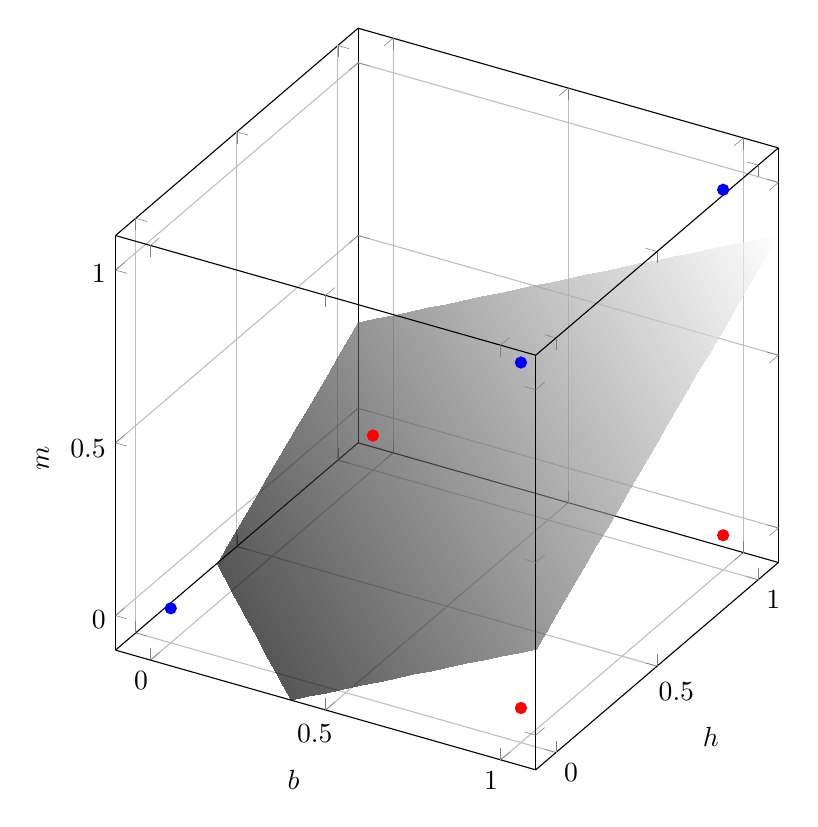
\begin{tikzpicture}
                \begin{axis}[
                    3d box,
                    width=10cm, height=11cm,
                    view={30}{30},
                    mark layer=like plot,
                    enlargelimits=false,
                    grid=major,
                    domain=-0.1:1.1,
                    zmin=-0.1, zmax=1.1,
                    xtick={0, 0.5, 1},
                    ytick={0, 0.5, 1},
                    ztick={0, 0.5, 1},
                    xlabel=$b$,
                    ylabel=$h$,
                    zlabel=$m$
                ]
                    \addplot3[only marks, red, on layer=background] table[row sep=crcr] {%
                        1 0 0\\
                        1 1 0\\
                        0 1 0\\
                    };

                    \addplot3[only marks, blue, on layer=foreground] table[row sep=crcr] {%
                        0 0 0\\
                        1 0 1\\
                        1 1 1\\
                    };

                    \addplot3[
                        surf,
                        shader=interp,
                        opacity=0.66,
                        colormap/blackwhite,
                        on layer=main
                    ] (x, {max(y, 0.3 - x)}, {0.5 * x + 0.5 * max(y, 0.3 - x) - 0.25});
                \end{axis}
            \end{tikzpicture}
        \end{figure}
    \end{solution}
\end{enumerate}

\newpage

\section{Predict your grade}

\begin{figure}[h]
    \centering
    \begin{tikzpicture}[node distance = 2cm]
        \node[state] (X1) {$x_1$};
        \node[state] (X2) [right of=X1] {$x_2$};
        \node[state] (X3) [right of=X2] {$x_3$};
        \node[state] (Y) [below of=X2] {$y$};

        \draw[arrow] (X1) to (X2);
        \draw[arrow] (X2) to (X3);
        \draw[arrow] (X1) to (Y);
        \draw[arrow] (X2) to (Y);
        \draw[arrow] (X3) to (Y);
    \end{tikzpicture}
\end{figure}

The hereabove Bayesian network represents how the final grade of a class is computed. In this model, $x_1$, $x_2$ and $x_3$ respectively denote the grades obtained by a student at the homework, project and exam. The teaching assistant that grades the homework also grades the project and the exam, which introduces a slight bias in the corrections. In particular, $x_2 \sim \N(a_1 x_1 + \mu_2, \sigma_2^2)$ and $x_3 \sim \N(a_2 x_2 + \mu_3, \sigma_3^2)$. Finally, $y \sim \N(a_3 x_1 + a_4 x_2 + a_5 x_3 + \mu_y, \sigma_y^2)$ stands for the final grade, which is a linear combination of the grades obtained by the student during the semester plus some Gaussian noise due to rounding errors. Answer the following questions about this model.

\begin{enumerate}
    \item Assuming the parameters of the model are known, what is the expected value of $y$ given $x_1$ and $x_2$.

    \begin{solution}
        Our task is to find the expectation
        \begin{equation*}
            \underset{p(y | x_1, x_2)}{\E} \sbk{y} = \int y \, p(y | x_1, x_2) \d{y} .
        \end{equation*}
        We know that
        \begin{equation*}
            p(y | x_1, x_2) = \int p(y | x_1, x_2, x_3) \, p(x_3 | x_1, x_2) \d{x_3} ,
        \end{equation*}
        where $p(y | x_1, x_2, x_3)$ and $p(x_3 | x_1, x_2)$ are linear Gaussian distributions given in the statement. Therefore, we have
        \begin{equation*}
            p(y | x_1, x_2) = \N\rbk*{a_3 x_1 + a_4 x_2 + a_5 (a_2 x_2 + \mu_3) + \mu_y, (a_5 \sigma_3)^2 + \sigma_y^2}
        \end{equation*}
        and, by definition of a Gaussian distribution,
        \begin{equation*}
            \underset{p(y | x_1, x_2)}{\E} \sbk{y} = a_3 x_1 + (a_4 + a_5 a_2) x_2 + a_5 \mu_3 + \mu_y.
        \end{equation*}
    \end{solution}

    \item Suppose now that the model's parameters are unknown. Given a learning set $d = \cbk{(x_{i,1}, x_{i,2}, y_i)}$ of $N$ independent and identically distributed points, determine the model that best describes $d$.

    \begin{solution}
        We know that the distribution of $y$ given $x_1$ and $x_2$ takes the form $\N(w_1 x_1 + w_2 x_2 + b, \sigma^2)$. Then, our task is to find the parameters $h = (w_1, w_2, b, \sigma)$ that maximize the likelihood of $d$, \ie{} the \emph{maximum likelihood estimation} (MLE)
        \begin{align*}
            h_{\text{MLE}} & = \arg \max_w p(d | h) \\
            & = \arg \max_h \prod_i p(x_i, y_i | h) \\
            & = \arg \max_h \log \prod_i p(x_i, y_i | h) \\ \displaybreak
            & = \arg \max_h \sum_i \log p(x_i, y_i | h) \\
            & = \arg \max_h \sum_i \log p(y_i | h, x_i) + \log p(x_i) \\
            & = \arg \max_h \sum_i \log p(y_i | h, x_i) \\
            & = \arg \max_h \sum_i \log \sbk*{\frac{1}{\sqrt{2 \pi \sigma^2}} \exp\rbk*{- \frac{(w^T x_i - y_i)^2}{2 \sigma^2}}} \\
            & = \arg \max_h \sum_i - \frac{1}{2} \log (2 \pi \sigma^2) - \frac{(w^T x_i - y_i)^2}{2 \sigma^2} \\
            & = \arg \min_h \log \sigma^2 + \frac{1}{\sigma^2} \frac{1}{N} \sum_i (w^T x_i - y_i)^2 ,
        \end{align*}
        where $x_i = \mat{x_{i,1} & x_{i,2} & 1}^T$ and $w = \mat{w_1 & w_2 & b}^T$. In the last expression, we observe that the summation term is independent from $\sigma$. Therefore,
        \begin{align*}
            w_{\text{MLE}} & = \arg \min_w \sum_i (w^T x_i - y_i)^2 ,
        \end{align*}
        which exactly corresponds to a \emph{linear regression} problem. Then, we find $w_{\text{MLE}}$ by canceling the gradient with respect to $w$, \ie{}
        \begin{align*}
            0 & = \nabla_{\!w} \sum_i (w^T x_i - y_i)^2 \\
            & = \nabla_{\!w} \sum_i (w^T x_i - y_i) (w^T x_i - y_i) \\
            & = \nabla_{\!w} \sum_i (w^T x_i)^2 + y_i^2 - 2 w^T x_i y_i \\
            & = \nabla_{\!w} \rbk*{w^T X^T X w + Y^T Y - 2 w^T X^T Y} \\
            & = 2 X^T X w - 2 X^T Y
        \end{align*}
        where $X = (x_i^T) \in \R^{N \times 3}$ and $Y = (y_i) \in \R^{N}$. Finally, we have
        \begin{alignat*}{2}
            && 0 & = X^T X w_{\text{MLE}} - X^T Y \\
            \Leftrightarrow \quad && w_{\text{MLE}} & = (X^T X)^{-1} X^T Y .
        \end{alignat*}
        Afterwards, we find $\sigma_{\text{MLE}}$ such that
        \begin{align*}
            \sigma_{\text{MLE}} & = \arg \min_\sigma \log \sigma^2 + \frac{\text{MSE}}{\sigma^2} \\
            & = \sqrt{\text{MSE}},
        \end{align*}
        where $\text{MSE}$ denotes the \emph{mean squared error}
        \begin{equation*}
            \frac{1}{N} \sum_i ({w_{\text{MLE}}}^T x_i - y_i)^2 .
        \end{equation*}
    \end{solution}
\end{enumerate}

\newpage

\section{Heteroscedastic linear regression}

What becomes the expression of the weight vector $w$ in the solution of question 2.2 if the noise is different for each sample? In particular, $y_i \sim N(w^T x, \sigma_i^2)$ and we know the values $\sigma_i$.

\newpage

\section{Ridge regression}

One can generalize the linear regression problem to the minimization problem
\begin{align*}
    w^* & = \arg \min_w \sum_i \ell(w^T x_i - y_i) ,
\end{align*}
where $\ell$ is a \emph{loss} function. Show that $\ell(x) = \abs{x}$ corresponds to assuming the noise follows a Laplace distribution in contrast to $\ell(x) = x^2$, which corresponds to assuming Gaussian noise.

\newpage

\section{Learning to play Pacman (August 2020)}

You observe a Grandmaster agent playing Pacman. How can you use the moves you observe to train your own agent?

\begin{enumerate}
    \item Describe formally the data you would collect, the inference problem you would consider, and how you would solve it.

    \item How would you design a neural network to control your agent? Define mathematically the neural network architecture, its inputs, its outputs, its parameters, as well as the loss you would use to train it.

    \item Discuss the expected performance of the resulting agent when \begin{enumerate*}
        \item the Grandmaster agent is optimal, and
        \item the Grandmaster agent is suboptimal.
    \end{enumerate*}
\end{enumerate}

\newpage

\section{Escape game (January 2022)}

A new virtual escape game came out, and you decide to play it. You arrive in a $5 \times 5$ grid world where each cell $(x, y)$ is a room with doors leading to the adjacent rooms. The game's goal is to reach the exit room as fast as possible, but its position is unknown. Furthermore, some regions of the world are full of riddles, and crossing rooms in these regions takes longer. Fortunately, a leaderboard with the players' best times is provided, starting from a few different rooms. Due to rounding errors, you assume that the best times reported in the leaderboard are measurements affected by additive Gaussian noise $\N(0, 1)$.

\begin{table}[h]
    \centering
    \begin{tabular}{c|cc}
        \toprule
        $i$ & Starting room & Measured best time \\
        \midrule
        1 & $(4, 5)$ & $2.0$ \\
        2 & $(5, 3)$ & $3.5$ \\
        3 & $(3, 3)$ & $4.5$ \\
        4 & $(4, 1)$ & $7.0$ \\
        5 & $(1, 2)$ & $8.5$ \\
        \bottomrule
    \end{tabular}
\end{table}

From the leaderboard, you wish to learn a heuristic approximating the best time to get to the exit, starting from room $(x, y)$. You decide to use a small neural network as approximator, described by the following parametric function,
\begin{align*}
    h(x, y; \phi) & = \text{ReLU}(x w_1 + y w_2 + w_3) + \text{ReLU}(x w_4 + y w_5 + w_6) \\
    \text{ReLU}(x) & = \max(x, 0) ,
\end{align*}
where $\phi = (w_1, w_2, w_3, w_4, w_5, w_6)$ is the set of parameters/weights of the neural network.

\begin{enumerate}
    \item Among the following sets of parameters ($A$, $B$ or $C$), which one would you use? Justify your answer.

    \begin{table}[h]
        \centering
        \begin{tabular}{c|cccccc}
            \toprule
            Set & $w_1$ & $w_2$ & $w_3$ & $w_4$ & $w_5$ & $w_6$ \\
            \midrule
            $\phi_A$ &$-1.5$ & $1$ & $4$ & $1$ & $-1.5$ & $6$ \\
            $\phi_B$ &$-1$ & $1.5$ & $3$ & $0$ & $-1$ & $4$ \\
            $\phi_C$ &$-2$ & $0.5$ & $4.5$ & $1.5$ & $0$ & $5$ \\
            \bottomrule
        \end{tabular}
    \end{table}

    \begin{solution}
        A set of parameters is better than another if it \enquote{explains} the data better, that is the likeliness of the data given the set of parameter is higher. Our task is to find the set of parameters that maximizes the likelihood of data under the assumed probability model, or maximum likelihood estimation (MLE). In our case, the data $d$ is the leaderboard and consists of independent position-time tuples $(x_i, y_i, t_i)$. From the statement, we gather that the (best) time $t$ is a function of the starting position $(x, y)$, approximated by a neural network $h(x, y; \phi)$. We also learn that our time measurements are affected by Gaussian noise.
        \begin{align*}
            \phi_{\text{MLE}} & = \arg\max_\phi p(d | \phi) \\
            & = \arg\max_\phi \prod_{i=1}^5 p(x_i, y_i, t_i | \phi) \\ \displaybreak
            & = \arg\max_\phi \prod_{i=1}^5 p(t_i | x_i, y_i, \phi) \, p(x_i, y_i) \\
            & = \arg\max_\phi \prod_{i=1}^5 \N(t; h(x, y; \phi), 1) \\
            & = \arg\max_\phi \sum_{i=1}^5 \log \sbk*{\frac{1}{\sqrt{2 \pi}} \exp \rbk*{-\frac{(t_i - h(x_i, y_i; \phi))^2}{2}}} \\
            & = \arg\min_\phi \sum_{i=1}^5 (t_i - h(x_i, y_i; \phi))^2
        \end{align*}
        Now that we have an objective $L(\phi)$ to minimize, we can evaluate it for each of the proposed sets and select the best one.
        \begin{align*}
            L(\phi_A) & = \sum_{i=1}^5 (t_i - h(x_i, y_i; \phi_A))^2 = (2.0 - 5.5)^2 + (3.5 - 6.5)^2 + \dots = 29.75 \\
            L(\phi_B) & = 35.75 \\
            L(\phi_C) & = 205.25
        \end{align*}
        The best set is $\phi_A$.
    \end{solution}

    \item You now assume a Gaussian prior $\N(0, 1)$ on each parameter. Which set of parameters in the table above would you now choose? Justify your answer.

    \begin{solution}
        Now that we hold a prior belief on the parameters, our task is to find the most likely set of parameters given the data, that is maximum a posteriori (MAP) estimation.
        \begin{align*}
            \phi_{\text{MAP}} & = \arg\max_\phi p(\phi | d) \\
            & = \arg\max_\phi p(d | \phi) p(\phi) \\
            & = \arg\max_\phi \prod_{i=1}^5 p(x_i, y_i, t_i | \phi) \prod_{j=1}^6 p(w_j) \\
            & = \arg\max_\phi \prod_{i=1}^5 \N(t; h(x, y; \phi), 1) \prod_{j=1}^6 \N(w_j; 0, 1) \\
            & = \arg\min_\phi \sum_{i=1}^5 (t_i - h(x_i, y_i; \phi))^2 + \underbrace{\sum_{j=1}^6 (w_j)^2}_{\norm{\phi}^2}
        \end{align*}
        Here again, we have an objective $L'(\phi)$ to minimize, which we evaluate for each of the proposed sets.
        \begin{align*}
            L'(\phi_A) & = L(\phi_A) + \sum_{j=1}^6 (w_j)^2 = 29.75 + (-1.5)^2 + (1)^2 + \dots = 88.25 \\
            L'(\phi_B) & = 65.0 \\
            L'(\phi_C) & = 257.0
        \end{align*}
        The best set is $\phi_B$.
    \end{solution}

    \item Discuss the procedure you would implement on a computer to find the optimal set of parameters, had the table above not been provided.

    \begin{solution}
        If the table is not provided, it is intractable to evaluate and compare all possible sets of parameters. However, we still want to minimize the MLE (or MAP) objective $L(\phi)$. We can improve a set of parameters $\phi$ by following the opposite of the objective's gradient $\nabla_{\! \phi} L(\phi)$, \ie{} performing \emph{gradient descent} steps
        \begin{equation*}
            \phi \gets \phi - \gamma \nabla_{\! \phi} L(\phi) ,
        \end{equation*}
        where $\gamma$ is the learning rate. As alternatives to gradient descent, one could mention genetic or Markov chain Monte Carlo (MCMC) algorithms.
    \end{solution}

    \item Using the heuristic $h(x, y; \phi_D)$ with $\phi_D = (-2, 1, 5, 0.5, -2, 7)$, apply $5$ iterations of the greedy search algorithm, starting from room $(1, 1)$.

    \begin{solution}
        The greedy search algorithm uses a priority queue as fringe. Our goal is to reach the exit as fast as possible. As our heuristic approximates the time to reach the exit from room $(x, y)$, we should prioritize rooms that have the lowest heuristic in our queue. We keep in our fringe the rooms that are reachable from the visited (closed set) rooms. For convenience, we denote rooms as a two-digit number $10 \times x + y$, annotate rooms with their priority $h(x, y; \phi_D)$ and prune visited rooms from the fringe.

        \begin{table}[H]
            \centering
            \begin{tabular}{l|l|c}
                \toprule
                Fringe (priority queue) & Closed & Expand \\
                \midrule
                11(9.5) & & 11 \\
                21(8.5), 12(8.0) & 11 & 12 \\
                21(8.5), 22(7.0), 13(6.5) & 11, 12 & 13 \\
                21(8.5), 14(7.0), 22(7.0), 23(5.5) & 11, 12, 13 & 23 \\
                21(8.5), 14(7.0), 22(7.0), 24(5.0), 33(4.5) & 11, 12, 13, 23 & 33 \\
                21(8.5), 14(7.0), 22(7.0), 32(6.0), 24(5.0), 43(3.5), 34(3.0) & 11, 12, 13, 23, 33 & 34 \\
                \bottomrule
            \end{tabular}
        \end{table}
    \end{solution}
\end{enumerate}

\newpage

\section*{Supplementary materials}

\begin{itemize}
    \item Heteroscedasticity

    \qrcode{https://en.wikipedia.org/wiki/Heteroscedasticity}

    \item Laplace distribution

    \qrcode{https://en.wikipedia.org/wiki/Laplace_distribution}

    \item Chapter 18 of the reference textbook.
\end{itemize}

\end{document}
